\documentclass[11pt,letterpaper]{article}
\usepackage[utf8]{inputenc}
\usepackage[english]{babel}
\usepackage{graphicx}
\usepackage{amsfonts}
\usepackage{multicol}
\usepackage{flushend}
\usepackage{float}
\usepackage{fancyhdr}
\usepackage{colortbl}
\usepackage{amssymb}
\usepackage[margin=0.5 in]{geometry}
\usepackage{hyperref}
\usepackage{amsmath}
\usepackage{diagbox, eqparbox, hhline}
\usepackage{amssymb}

\renewcommand{\theequation}{\arabic{equation}}
\newcounter{neq}

\begin{document}
\setlength{\unitlength}{1cm}
\thispagestyle{empty}
\begin{picture}(18,4)
\put(0.5,0.2){
\includegraphics[scale=.35]{./img/unam1}}
\put(14.5,0){
\includegraphics[scale=.4]{./img/fciencias1}}
\end{picture}

\begin{center}
\textbf{{\LARGE Universidad Nacional Autónoma de México}}\\[0.2cm]
\textbf{{\LARGE Facultad de Ciencias\\Castro Mejia Jonatan Alejandro 314027687\\Leyva Castillo Luis Angel 314050577\\~\\Rosado Cabrera Diego 314293804}}\\[0.2cm]
\end{center}
\section{XSS}
\begin{center}
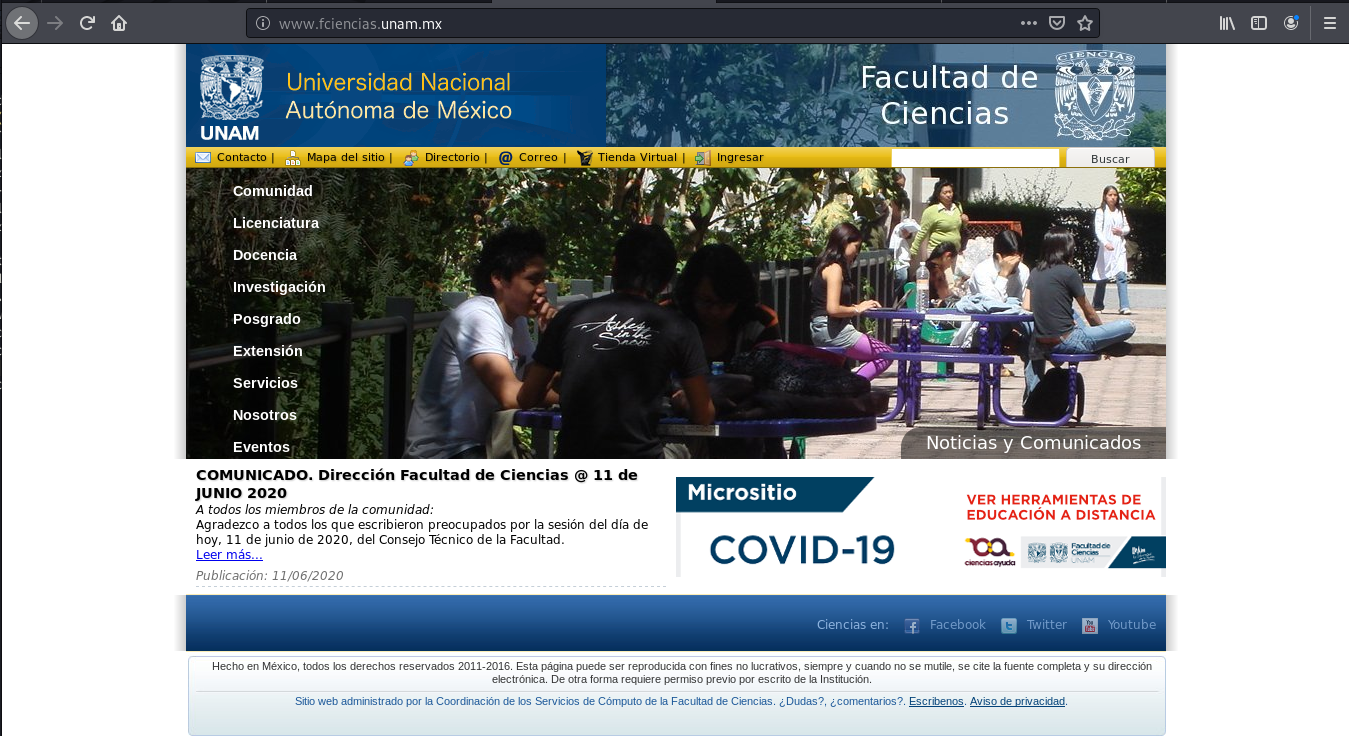
\includegraphics[scale=.4]{./Img/img0.png}
\end{center}~\\~\\~\\
\begin{center}
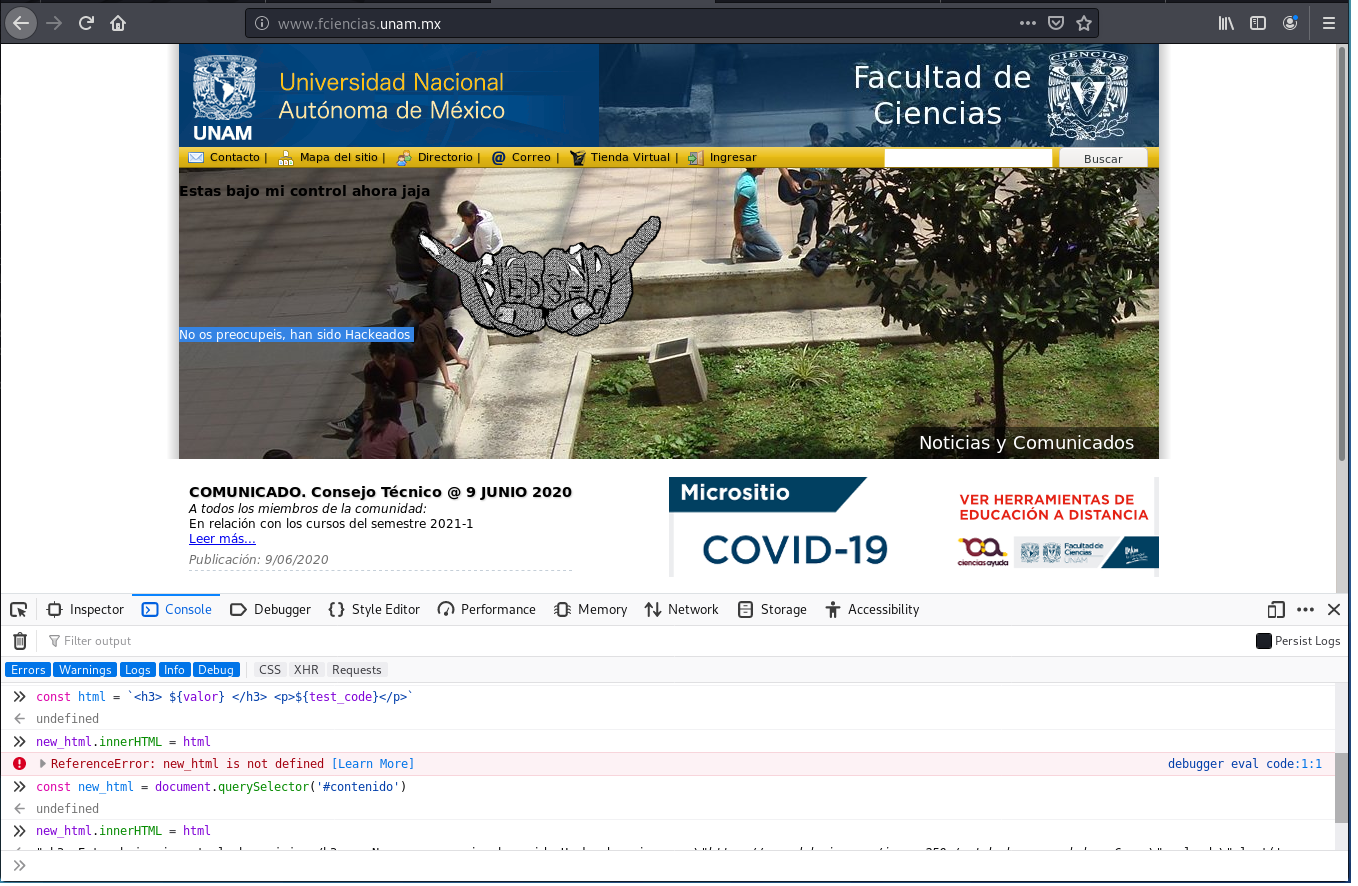
\includegraphics[scale=.4]{./Img/img1.png}
\end{center}~\\~\\~\\
\begin{center}
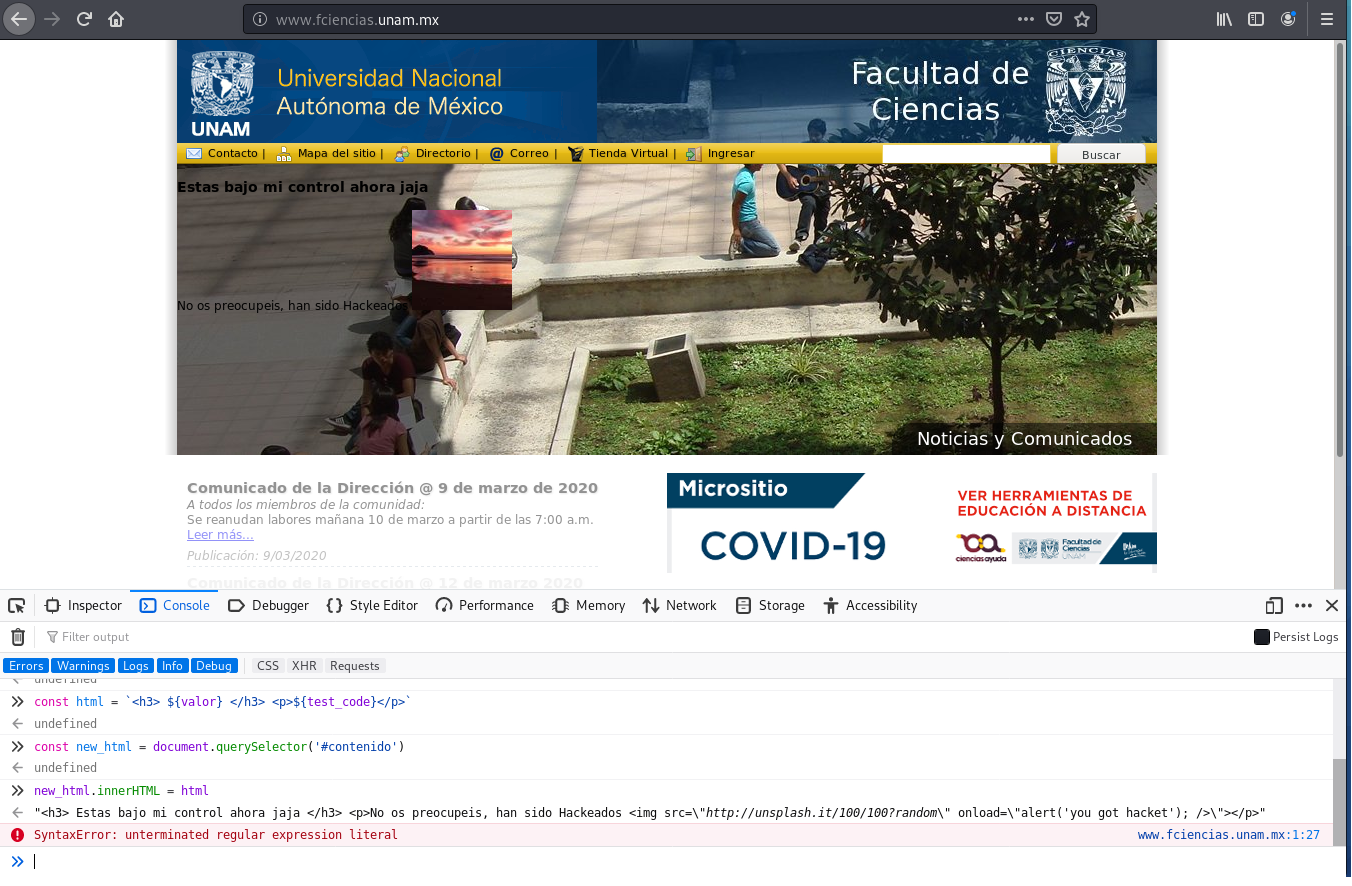
\includegraphics[scale=.4]{./Img/img2.png}
\end{center}~\\~\\~\\
\section{SQL Injection}
%Para XSS, encontrar un sitio web que presente esta vulnerabilidad, e inyectar una imagen de un servicio remoto, así como mostrar que se puede ejecutar código JavaScript ajeno a la página web original. Incluir captura de pantalla del sitio web que muestre el antes y el después de la ejecución del código XSS.
%sPara SQLinjection, utilizar la herramienta sqlmap. Con base en la documentación de sqlmap y el análisis de los comandos vistos en clase, obtener el usuario y contraseña para el sitio:
\end{document}